\chapter{Simulation Results}\label{sec:chapter}

\section{Simulation Setup}\label{sec:section}

\begingroup
To model different adversarial attacks we mainly rely on Python 3.6 \cite{Python} and Tensorflow 1.7 \cite{Tensorflow}.
Tensorflow is a math library used for machine learning applications such as neural networks. The framework makes
it easy to develop DNNs with more than one hidden layer. This is especially helpful for more complex DNN architectures.
Furthermore, tensorflow provides a lot of necessary algorithms for backpropagation out-of-the-box. Therefore, the
development time gets heavily reduced.

The project itself is structured in a modular form. The datasets object enables access to the CIFAR, MNIST, SET14
and STL10 dataset. CIFAR (32x32) was published by the Canadian Institute for Advanced Research and is mainly used for object
classification. MNIST (28x28) contains a database of handwritten digits in black and white. It is one of the most
basic datasets, primarily used for character recognition. STL10 is a higher resolution (96x96)
object classification dataset. SET14 contains a selected set of popular test images.
Models used in this project are defined in the $models.json$ file. Adversarial examples are
generated in the $adversarial.py$ file. Norms and models can be selected using commands specified in the parser object. Final
results are saved in $csv$ and $eps$ files stored in the $results$ folder.
\endgroup

\begingroup
To test the effectiveness of adversarial attacks presented in previous sections, various models and datasets are used.
For comparibility reasons, the focus was set on autoencoders reproducing an identity function. Furthermore, attacks
were tested against convolutional AEs like colorization or super-resolution models.
An overview of the models and datasets used in the simulations is provided
by \autoref{ModelTable}.

FCNN is a fully-connected model, which is trained based on grayscale images of the MNIST dataset. The trained network
has a compression rate of 96\%. FCNN2 is similarly trained for the MNIST dataset, but uses convolutional layer with
a fully-connected layer in the center of the ntwork. For CIFAR, FCNN3 is trained as a fully-connected network with a
compression rate of 50\%. As an activation function all layers in the FCNN networks except the output layer use ReLu.
The output is provided using a Sigmoid function. ReLu offers better convergence properties than formerly used
TanH or Sigmoid functions. This is due to the higher linearity of the ReLu function.
The training of all the FCNN models was performed using an Adam Optimizer with a decreasing learning
rate $\alpha$.

AEN\_STL10 relies entirely on convolutional layers. The same holds true for KOALA \cite{KoalaModel} and C\_DCSCN
\cite{SuperModel}. Each convolutional layer in both models uses a ReLu activation function. For the super-resolution
model LeakyReLu is used to avoid the "dying ReLu" problem. Outputs of these
autoencoders are transformed to be plotted in RGB afterwards. For instance, the KOALA model requires the CbCr channel
to be merged with the Y color channel.

C\_DCSCN is trained to return an upsampled version of an input image. The underlying model first uses a bicubic interpolation
to approximate the super-resolution image. Afterwards, a residual CNN is created that focusses on learning the
residual between the original image and bicubic interpolation of the low resolution and high resolution
image \cite{SuperModel,SuperModel2}. An overview of the structure of the C\_DCSCN model is given by \autoref{c_dcscn_network_structure}.
Training of C\_DCSCN was performed using dropout. This technique removes a certain
portion (dropout rate) of nodes during training. This avoids training only a small set of the topology for the actual
classification or regression problem.
\endgroup


\begin{table}[]
\centering
\def\arraystretch{1.8}
\caption{Models and Datasets}
\label{ModelTable}
\begin{tabular}{|c|c|c|c|c|}
\hline
\textbf{Model} & \textbf{Dataset} & \textbf{Description} & \textbf{Input} & \textbf{Output} \\ \hline
FCNN           & MNIST            & Autoencoder          & Y              & Y               \\ \hline
FCNN2          & MNIST            & Autoencoder          & Y              & Y               \\ \hline
FCNN3          & CIFAR            & Autoencoder          & RGB            & RGB             \\ \hline
AEN\_STL10     & STL10            & Autoencoder          & RGB            & RGB             \\ \hline
KOALA          & STL10            & Colorization         & Y              & CbCr            \\ \hline
C\_DCSCN       & SET14            & Super-Resolution     & Y              & Y               \\ \hline
\end{tabular}
\end{table}


\begin{figure}[ht] % "[t!]" placement specifier just for this example
	\centering
\includegraphics[width=.7\linewidth]{\detokenize{c_dcscn_network_structure}}
\caption{C\_DCSCN structure as shown in \cite{SuperModel}}
\label{c_dcscn_network_structure}
\end{figure}



\begingroup
The Peak Signal-To-Noise Ratio (PSNR) describes the ratio between the maximum possible signal power and the power of the noise.
Most commonly the ratio is defined by \ref{07_psnr_definition} and \ref{07_mse_definition} \cite{PSNRConversion}. In these equations MAX defines
the maximum pixel value, $N$ the amount of given pixels and channels and $\hat{x}$ the noisy image itself.
\endgroup

\begin{equation}
\begin{aligned}
	\text{PSNR} = 10 \cdot log_{10} (\frac{\text{MAX}^2}{\text{MSE}})
\end{aligned}
\label{07_psnr_definition}
\end{equation}

\begin{equation}
\begin{aligned}
	\text{MSE} = \frac{1}{N} \sum_{i=1}^N (\hat{x}_i - x_i)^2
\end{aligned}
\label{07_mse_definition}
\end{equation}

\begingroup
Unfortunately, the input perturbation is limited by the $p$-norm $\lvert\lvert \bm{\eta} \rvert\rvert_p \leq \epsilon$ and only
$\epsilon$ is given. Therefore, the upper boundary needs to be found in terms of the $l_2$-norm.
\endgroup

\begin{equation}
\begin{aligned}
p=1: \quad & \lvert\lvert \bm{\eta} \rvert\rvert_{1 \rightarrow 2} \leq \epsilon \\[10pt]
p=2: \quad & \lvert\lvert \bm{\eta} \rvert\rvert_{2 \rightarrow 2} \leq \epsilon \\[10pt]
p=\infty: \quad & \lvert\lvert \bm{\eta} \rvert\rvert_{\infty \rightarrow 2} \leq \epsilon^2 N
\end{aligned}
\label{operator_epsilon}
\end{equation}

\begingroup
Using these approximations and setting $\text{MAX} = 1$ leads to the following PSNRs.
\endgroup

\begin{equation}
\begin{aligned}
p=1: \quad & \text{PSNR} = 10 \cdot log_{10} (\frac{N}{\epsilon}) \\[10pt]
p=2: \quad & \text{PSNR} = 10 \cdot log_{10} (\frac{N}{\epsilon}) \\[10pt]
p=\infty: \quad & \text{PSNR} = 10 \cdot log_{10} (\frac{N}{\epsilon^2}) = -20 \cdot log_{10} (\epsilon)
\end{aligned}
\label{psnr_simplify}
\end{equation}

\begingroup
Super-resolution and colorization models sometimes do not stay within the same color spaces. To convert between
the YCbCr and RGB color space the following conversion is necessary \cite{YCbCrConversion}. RGB values follow
through the inverse.
\endgroup

\begin{equation}
\begin{bmatrix}
Y \\
Cb \\
Cr
\end{bmatrix}
=
\begin{bmatrix}
0 \\
128 \\
128
\end{bmatrix}
+
\begin{bmatrix}
0.299 & 0.587 & 0.114 \\
-0.168736 & -0.331264 & 0.5 \\
0.5 & -0.41868 & -0.081312
\end{bmatrix}
\begin{bmatrix}
R \\
G \\
B
\end{bmatrix}
\end{equation}

\section{Results}\label{sec:section}

\begingroup
All the test results, which were observed during this thesis, can be found in the appendix.
The experiments are conducted using an $\epsilon$ value between 0.1 and 0.7 with a linear step size of 0.1.
Therefore, a wide range of input perturbation changes is covered.
In the source code and figures $pixel$ describes the quadratic single subset attack, if not further specified.
The simulations have shown that the effectiveness of adversarial examples highly depends on the chosen model.
The linear perturbation solution for a number of iterations $S$ is given by $lin$-$l_p$-$S$. $quad$-$l_p$-$1$ denotes the quadratic
solution. Since the conducted experiments are primarily image based, PSNR is used as a performance metric.

To compare different adversarial attacks $rand$-$l_p$ is used as a random benchmark under a $l_p$ constraint. For $p=2$
the entries from the perturbation change $\bm{\eta}$ are independently drawn from a Gaussian distribution and divided
by the respective $l_2$-norm. In the case of $p = \infty$, independent Bernoulli experiments are conducted for each entry
of $\bm{\eta}$ to determine the sign of $\epsilon$.
\endgroup


\begin{figure}[!htb]
	\begin{minipage}{0.45\textwidth}
		\centering
		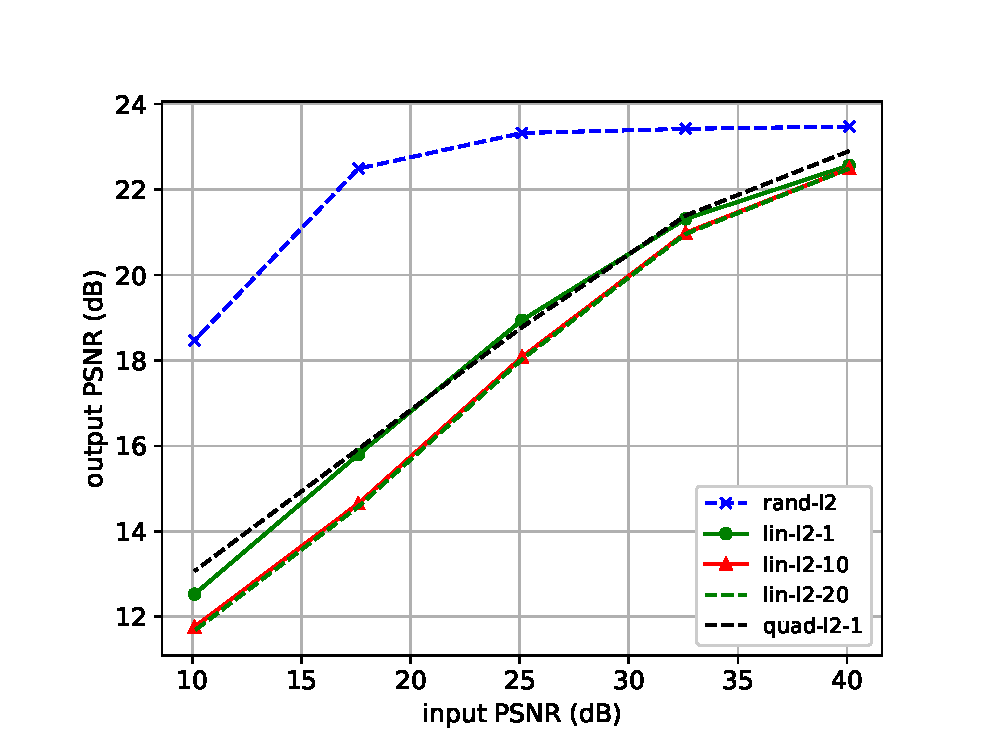
\includegraphics[width=.95\linewidth]{\detokenize{./images/figures/fcnn_fig_mnist_l2}}
		\caption{FCNN PSNR Figure ($l_2$-Norm)}
		\label{fcnn_l2_figure}
	\end{minipage}\hfill
	\begin {minipage}{0.45\textwidth}
		\centering
	 	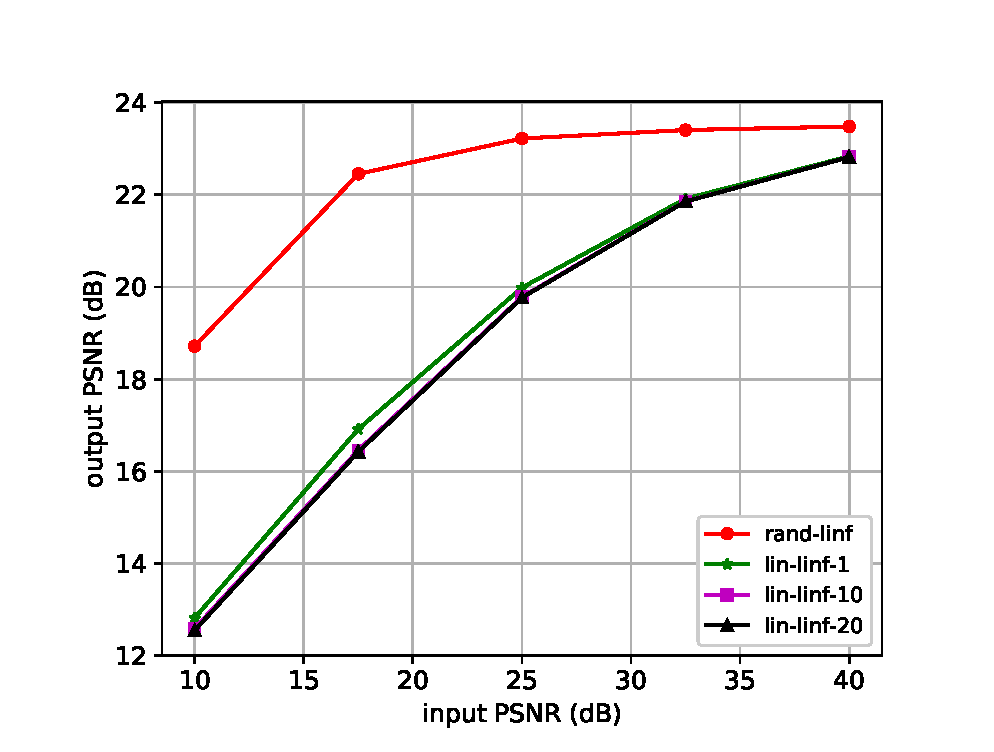
\includegraphics[width=.95\linewidth]{\detokenize{./images/figures/fcnn_fig_mnist_linf}}
		\caption{FCNN PSNR Figure ($l_\infty$-Norm)}
		\label{fcnn_linf_figure}
	\end{minipage}
\end{figure}


\begingroup
For the FCNN network \autoref{fcnn_l2_figure} and \autoref{fcnn_linf_figure} display the linear and quadratic
perturbation change under a $l_2$ and $l_\infty$ constraint. In this case,
the $l_2$-solution slightly outperforms the $l_\infty$ solution due to higher degrees
of freedom in the $l_2$-norm. The maximum output change for the FCNN network diverges around 6.5 dB from the random
benchmark under the $l_2$-norm constraint. For the $l_\infty$-norm the PSNR change is only 6 dB.
\endgroup


\begin{figure}[!htb]
	\begin{minipage}{0.45\textwidth}
		\centering
		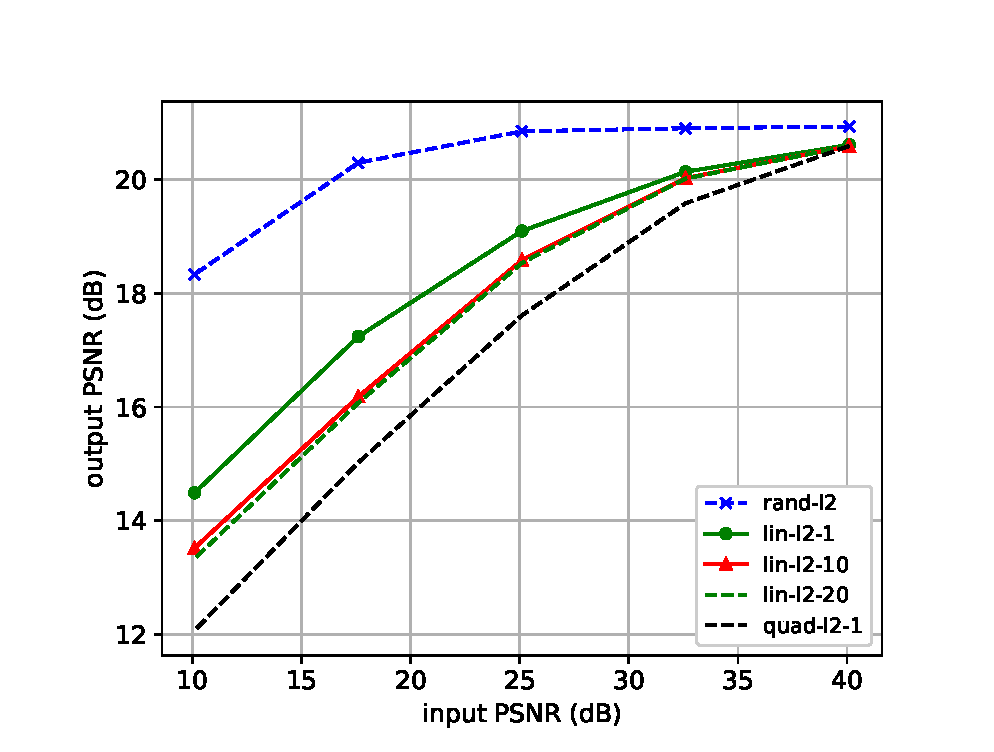
\includegraphics[width=.95\linewidth]{\detokenize{./images/figures/fcnn2_fig_mnist_l2}}
		\caption{FCNN2 PSNR Figure ($l_2$-Norm)}
		\label{fcnn2_l2_figure}
	\end{minipage}\hfill
	\begin {minipage}{0.45\textwidth}
		\centering
	 	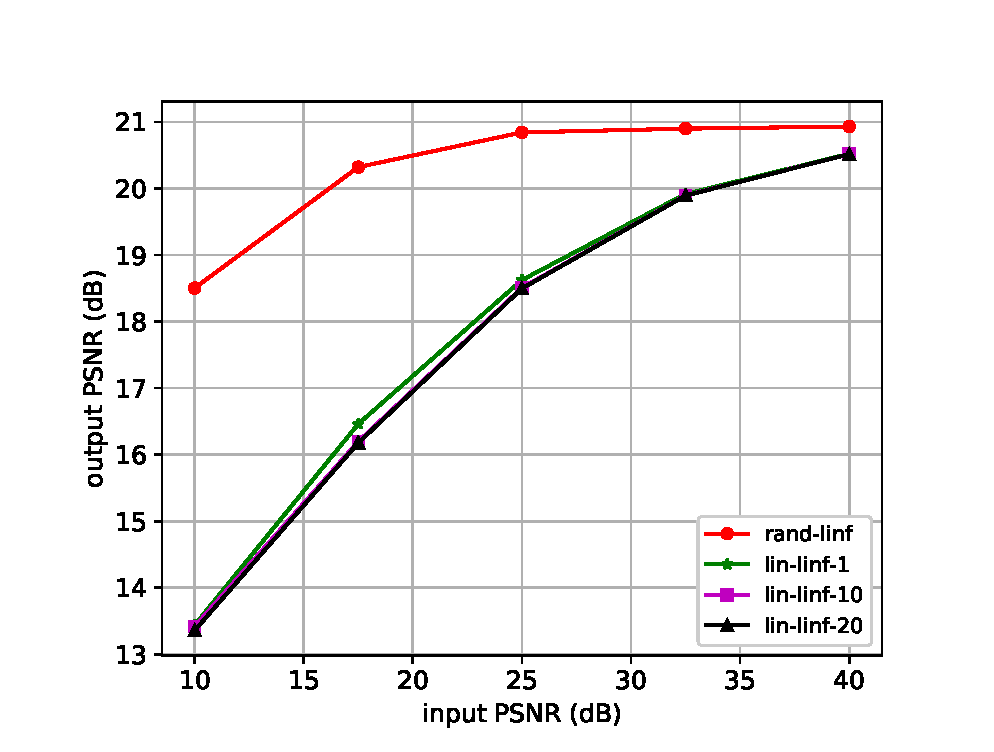
\includegraphics[width=.95\linewidth]{\detokenize{./images/figures/fcnn2_fig_mnist_linf}}
		\caption{FCNN2 PSNR Figure ($l_\infty$-Norm)}
		\label{fcnn2_linf_figure}
	\end{minipage}
\end{figure}


\begingroup
The FCNN2 network yields similar results. The best adversarial examples are provided by the quadratic solution with a 6.2 dB lower PSNR.
In contrast to the results from the FCNN network, the linear solutions provide significantly worse results than the quadratic solution. 20 iterations
of the linear closed form solution using the $l_2$ constraint are around 1 dB less effective than one iteration of the quadratic solution.
20 iterations also perform only 0.1 dB better than 10 iterations. For the $l_\infty$-norm the change between multiple iterations is even less noticable.
\endgroup

\begin{figure}[!htb]
	\begin{minipage}{0.45\textwidth}
		\centering
		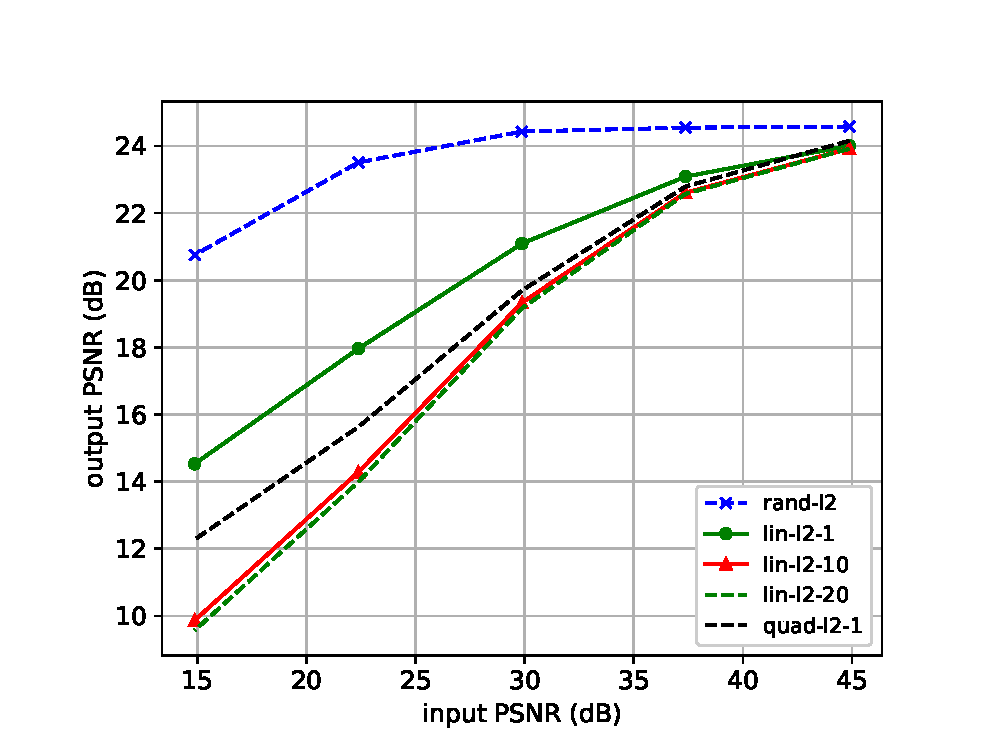
\includegraphics[width=.95\linewidth]{\detokenize{./images/figures/fcnn3_fig_cifar_l2}}
		\caption{FCNN3 PSNR Figure ($l_2$-Norm)}
		\label{fcnn3_l2_figure}
	\end{minipage}\hfill
	\begin {minipage}{0.45\textwidth}
		\centering
	 	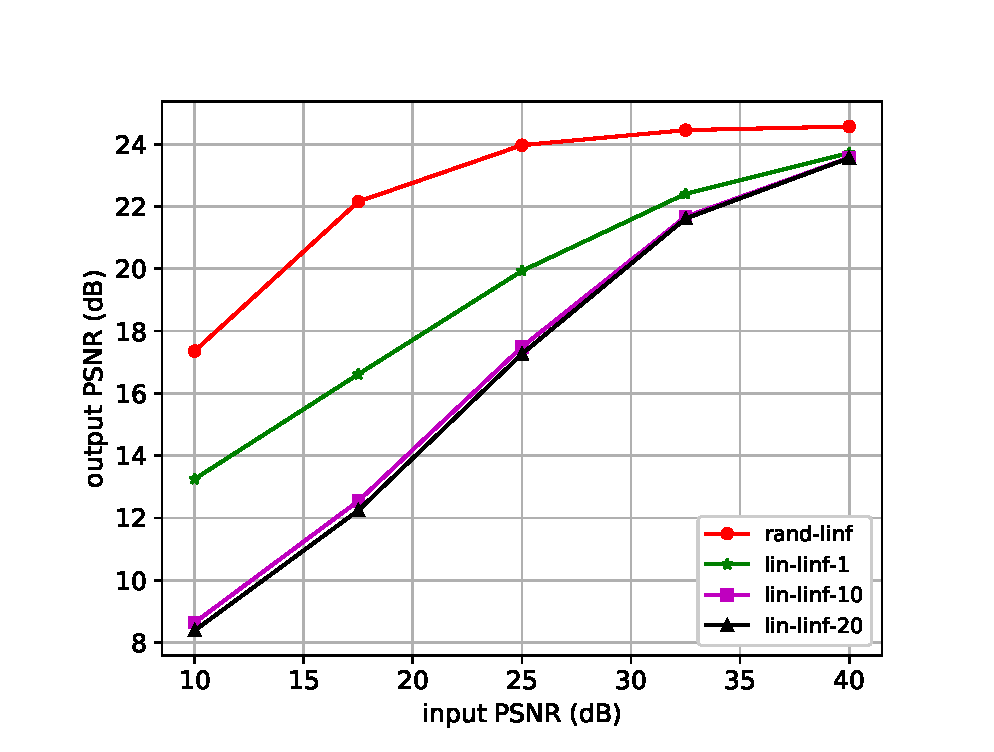
\includegraphics[width=.95\linewidth]{\detokenize{./images/figures/fcnn3_fig_cifar_linf}}
		\caption{FCNN3 PSNR Figure ($l_\infty$-Norm)}
		\label{fcnn3_linf_figure}
	\end{minipage}
\end{figure}

\begingroup
For FCNN3 the experiments' results are shown in \autoref{fcnn3_l2_figure} and \autoref{fcnn3_linf_figure}.
The maximum PSNR change from a random benchmark is 11 dB. In this case the linear solution
outperforms the quadratic solution by 2 dB for 10 and 20 iterations. The higher number of dimensions in the CIFAR
dataset seems to benefit the iterative solution. Generally, it is noticable that lower PSNR input values relate
to lower PSNR output values. This is sensible since lower PSNR values are directly connected to higher $\epsilon$ values
through the MSE.
\endgroup

\begin{figure}[!htb]
	\begin{minipage}{0.45\textwidth}
		\centering
		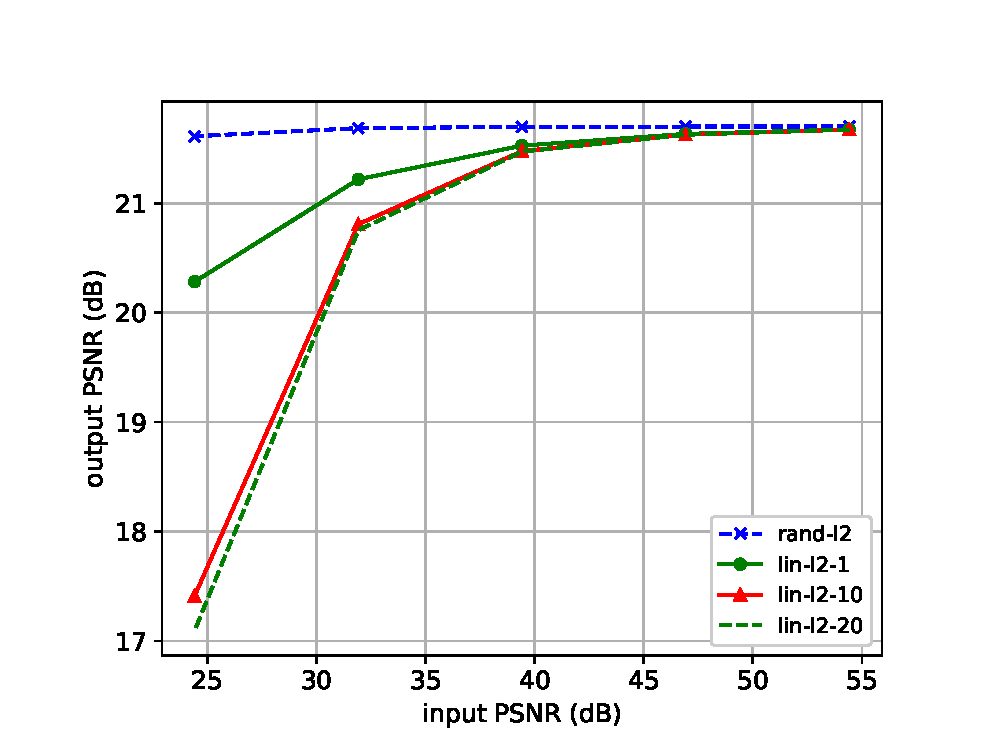
\includegraphics[width=.95\linewidth]{\detokenize{./images/figures/aen_stl10_fig_stl10_l2}}
		\caption{AEN\_STL10 PSNR Figure ($l_2$-Norm)}
		\label{aen_stl10_l2_figure}
	\end{minipage}\hfill
	\begin {minipage}{0.45\textwidth}
		\centering
	 	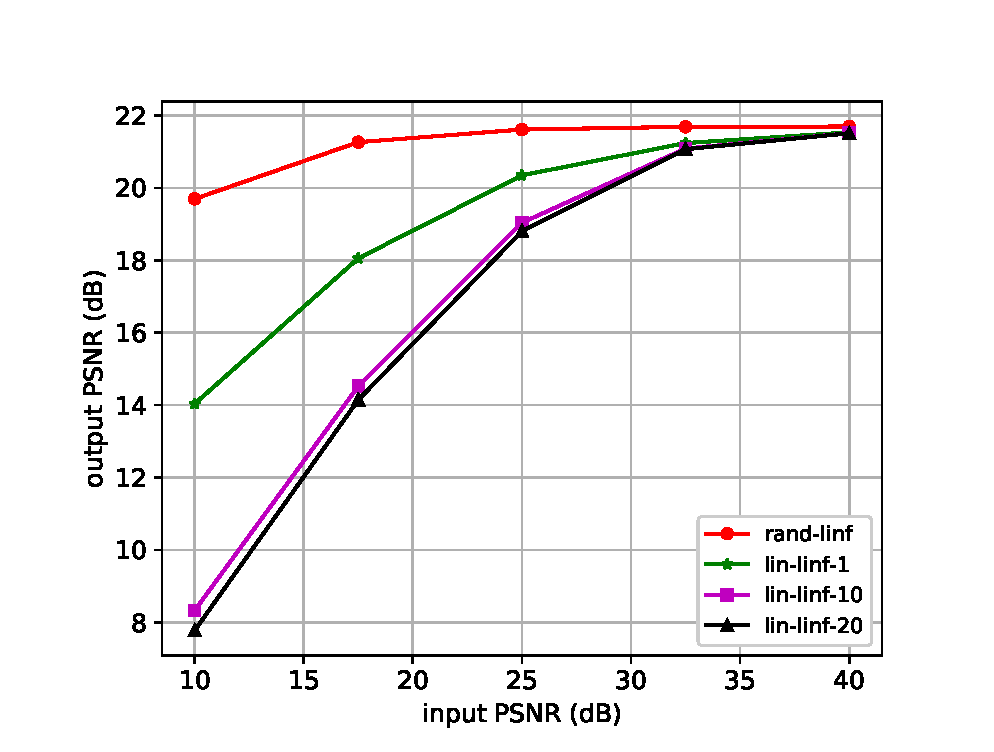
\includegraphics[width=.95\linewidth]{\detokenize{./images/figures/aen_stl10_fig_stl10_linf}}
		\caption{AEN\_STL10 PSNR Figure ($l_\infty$-Norm)}
		\label{aen_stl10_linf_figure}
	\end{minipage}
\end{figure}

\begingroup
AEN\_STL10 performs similar to previously discussed networks, but shows a rapid decline for higher $\epsilon$ values.
An input PSNR change from 25 dB to 33 dB leads to an output PSNR change of more than 3 dB.
The iterative improvement from 10 to 20 iterations is less than 0.5 dB for the $l_2$ and $l_\infty$ solution.
\endgroup


\begin{figure}[!htb]
	\begin{minipage}{0.45\textwidth}
		\centering
		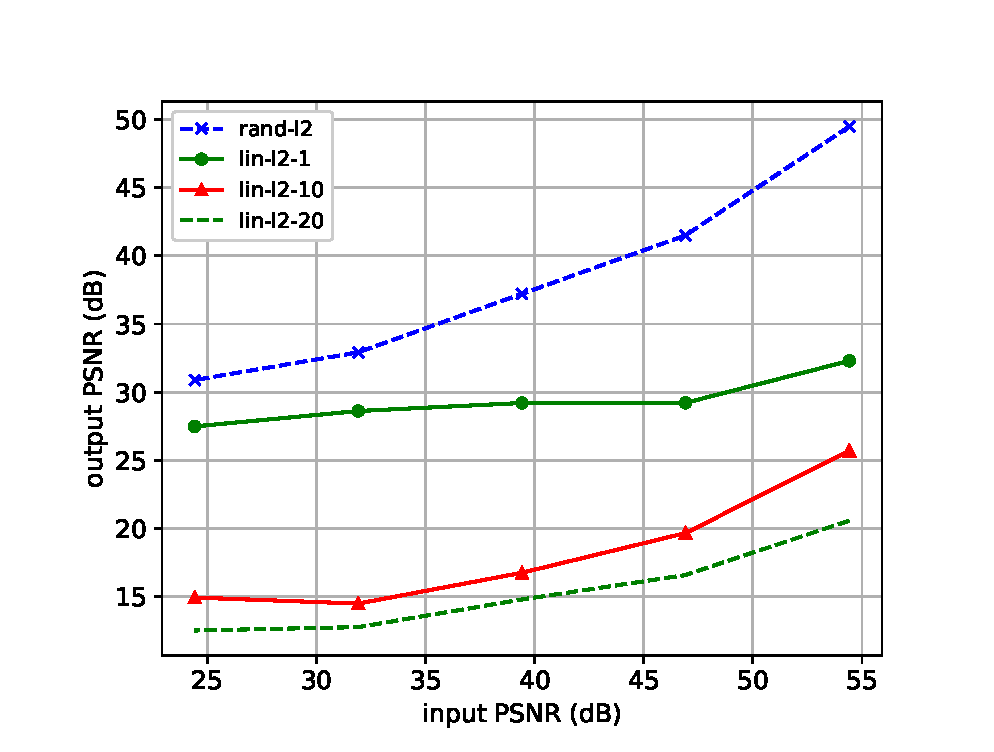
\includegraphics[width=.95\linewidth]{\detokenize{./images/figures/koala_fig_stl10_l2}}
		\caption{KOALA PSNR Figure ($l_2$-Norm)}
		\label{koala_l2_figure}
	\end{minipage}\hfill
	\begin {minipage}{0.45\textwidth}
		\centering
	 	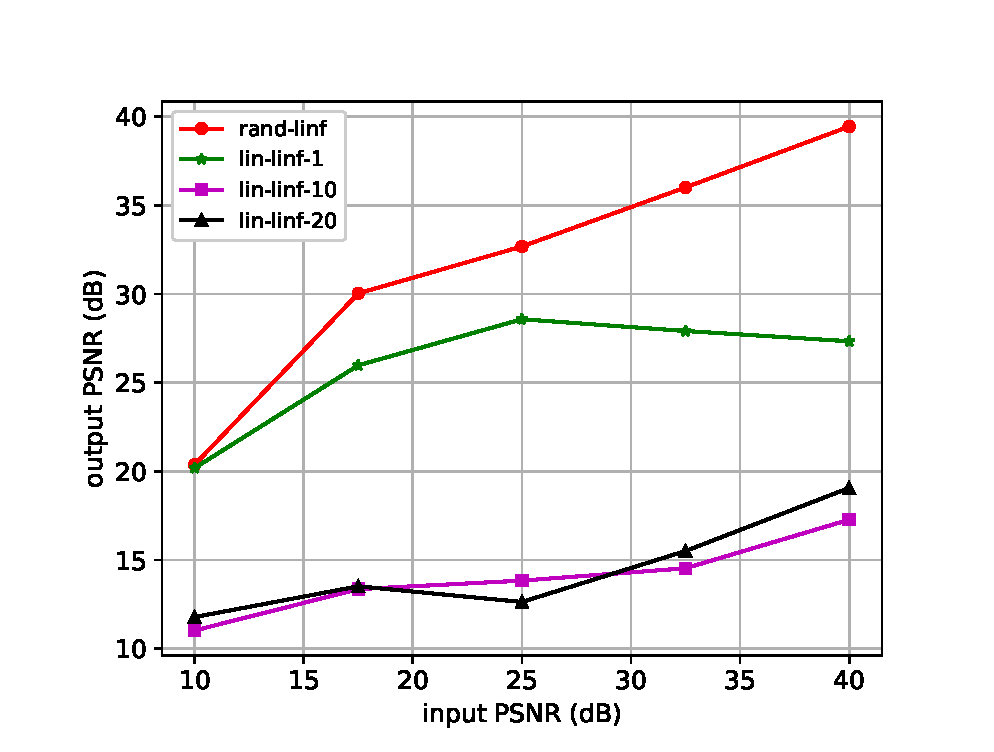
\includegraphics[width=.95\linewidth]{\detokenize{./images/figures/koala_fig_stl10_linf}}
		\caption{KOALA PSNR Figure ($l_\infty$-Norm)}
		\label{koala_linf_figure}
	\end{minipage}
\end{figure}

\begingroup
The PSNR graphs for the colorization model KOALA vary greatly from previously discussed models. Instead of an increasingly
worse output for higher $\epsilon$ values the output stagnates for $l_2$ and $l_\infty$. This is caused by merging the gray
color channel with the output layer without any modifications. Furthermore, it is noteworthy that $l_\infty$ shows some
instabilities for 10 and 20 iterations.
\endgroup

\begin{figure}[!htb]
	\begin{minipage}{0.45\textwidth}
		\centering
		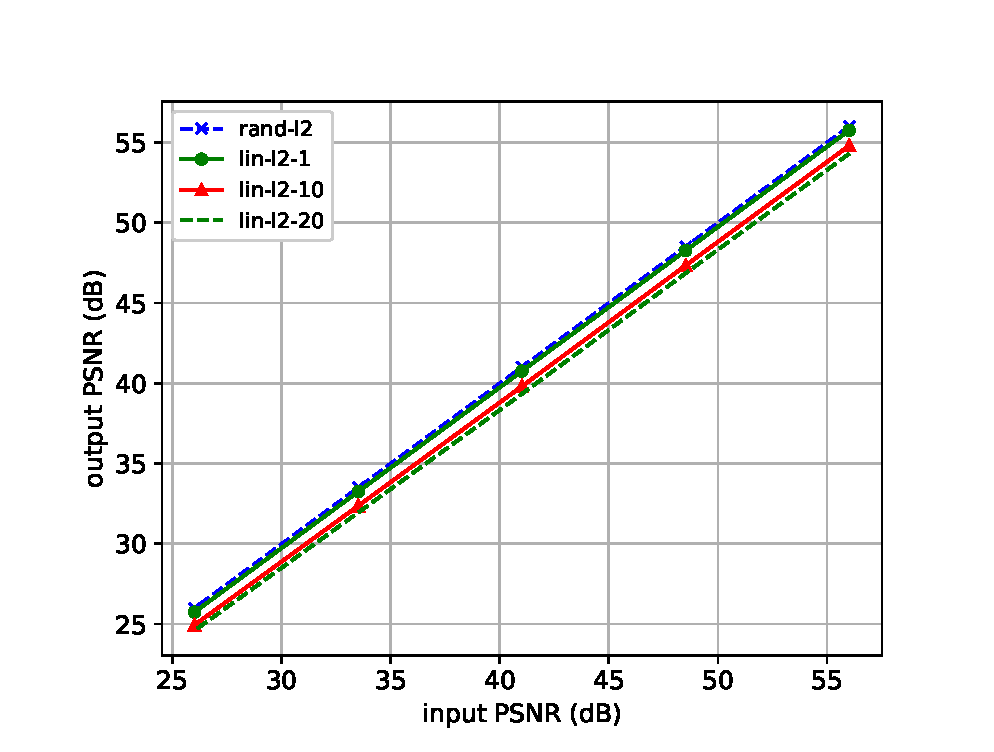
\includegraphics[width=.95\linewidth]{\detokenize{./images/figures/c_dcscn_fig_set14_l2}}
		\caption{C\_DCSCN PSNR Figure ($l_2$-Norm)}
		\label{c_dcscn_l2_figure}
	\end{minipage}\hfill
	\begin {minipage}{0.45\textwidth}
		\centering
	 	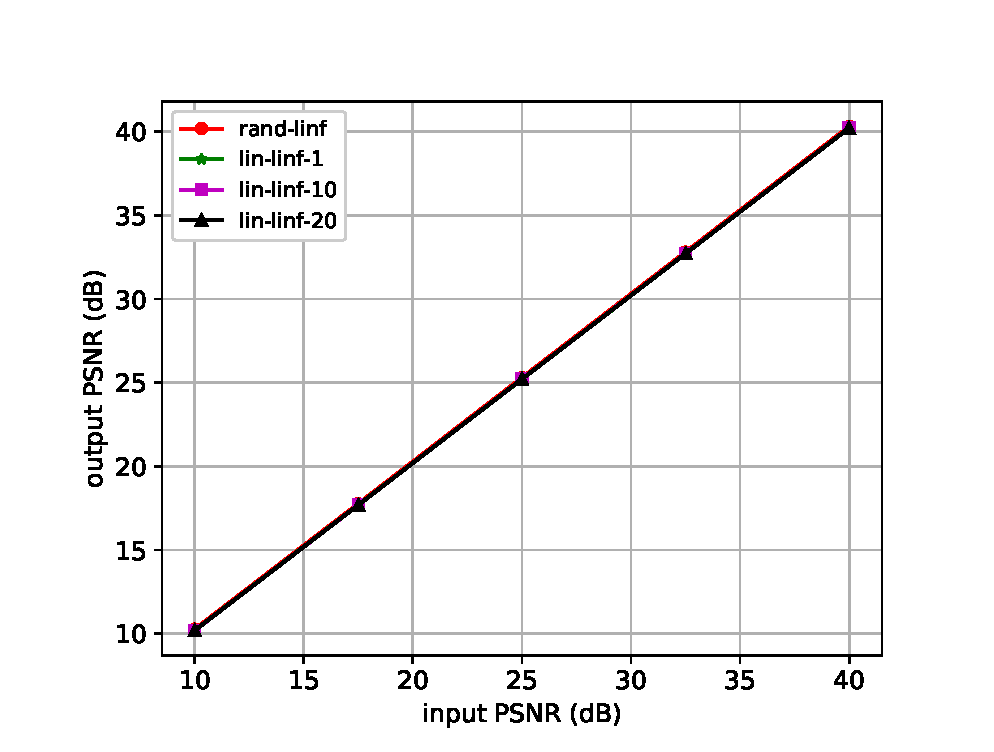
\includegraphics[width=.95\linewidth]{\detokenize{./images/figures/c_dcscn_fig_set14_linf}}
		\caption{C\_DCSCN PSNR Figure ($l_\infty$-Norm)}
		\label{c_dcscn_linf_figure}
	\end{minipage}
\end{figure}


\begingroup
Similarly to KOALA, C\_DCSCN has a relatively stable PSNR change for different $\epsilon$ values. In this case the
small impact of adversarial examples is most likely caused by the bicubic interpolation and dropout training used
in training the network. Since the DNN is only used to calculate a residual to the bicubic interpolation the impact
of adversarial examples is low.
\endgroup

\begingroup
In general, the quadratic and linear solution for 20 iterations lie within a range of 2 dB from each other. Therefore,
the impact of more than 10 iterations seems to be low. However, successive linearizations heavily improve the
performance of linear adversarial attacks. Linear solutions seem to perform better for datasets
with multiple color channels like CIFAR. The quadratic solution only performed slightly better than
the linear solution for the MNIST dataset.
Despite this fact, the quadratic solution can be performed using less iterations and can therefore yield faster results if the memory requirements for the jacobians
are met.

One of the most notable examples for the MNIST dataset is provided by \autoref{fcnn2_examples} for a PSNR
of 32.50 and the FCNN2 network. It can be observed that FCNN2 is able to denoise random input changes, but fails for linear
perturbation changes. For STL10 the most notable changes can be shown using the KOALA network in \autoref{koala_examples}.
The output images are completely distorted from the original image.
For CIFAR \autoref{fcnn3_examples} shows perturbation changes for the FCNN3 network. The example images also show that
output changes are not uniformly distributed.
\endgroup


\begin{figure}[ht] % "[t!]" placement specifier just for this example
	\centering
\includegraphics[width=.7\linewidth]{\detokenize{koala_l2_39.42_exp}}
\caption{KOALA $l_{2}$-norm Examples for PSNR of 39.42}
\label{koala_examples}
\end{figure}


\begin{figure}[ht] % "[t!]" placement specifier just for this example
	\centering
\includegraphics[width=.7\linewidth]{\detokenize{fcnn2_linf_32.50_exp}}
\caption{FCNN2 $l_{\infty}$-norm Examples for PSNR of 32.50}
\label{fcnn2_examples}
\end{figure}

\begin{figure}[ht] % "[t!]" placement specifier just for this example
	\centering
\includegraphics[width=.7\linewidth]{\detokenize{fcnn3_l2_22.37_exp}}
\caption{FCNN3 $l_{2}$-norm Examples for PSNR of 22.37}
\label{fcnn3_examples}
\end{figure}


\begingroup
Apart from strictly linear and quadratic solutions this thesis has also provided different multiple pixel attacks.
In this case $rand$-$T$, $lin$-$T$ and $pixel$-$T$ denote multiple subset attacks that change $T$ pixels.
Since all experiments were image based, subset and pixel can be used synonymously in the following paragraphs.
For $rand$-$T$ a set of pixels is randomly drawn and the values determined based on the respective norm constraint.
\autoref{fcnn_single_figure} and \autoref{fcnn2_single_figure} show multiple single pixel attacks for 100
changed subsets. Most notably the quadratic multiple subset attack performs better than the linear attack for
all chosen models and datasets. This is caused by missing iteration steps for the linear solution.
$pixel$ and $pixel$-$100$ define the different quadratic adversarial attacks. It can
be observed that a higher number of attacked subsets leads to a lower PSNR. Furthermore, higher $\epsilon$
values can be directly related to a lower PSNR. Some adversarial examples for FCNN3 are provided by
\autoref{fcnn3_single_examples}.
\endgroup


\begin{figure}[!htb]
	\begin{minipage}{0.45\textwidth}
		\centering
		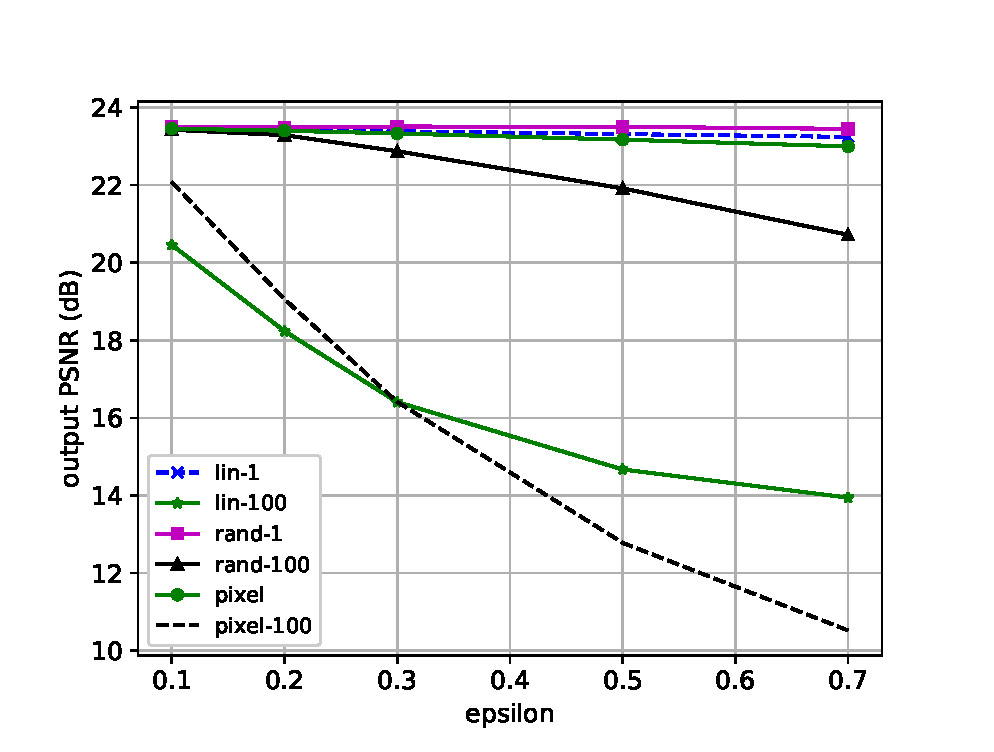
\includegraphics[width=.95\linewidth]{\detokenize{./images/figures/fcnn_fig_mnist_pixel}}
		\caption{FCNN PSNR Figure (Single Subset Attack)}
		\label{fcnn_single_figure}
	\end{minipage}\hfill
	\begin {minipage}{0.45\textwidth}
		\centering
	 	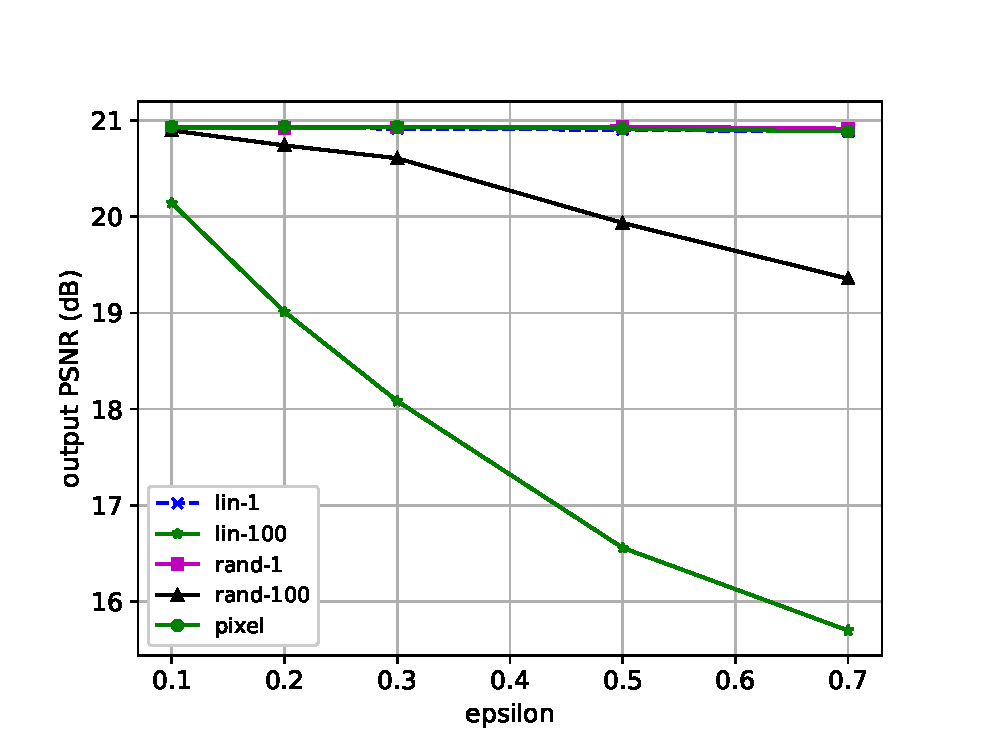
\includegraphics[width=.95\linewidth]{\detokenize{./images/figures/fcnn2_fig_mnist_pixel}}
		\caption{FCNN2 PSNR Figure (Single Subset Attack)}
		\label{fcnn2_single_figure}
	\end{minipage}
\end{figure}


\begin{figure}[ht] % "[t!]" placement specifier just for this example
	\centering
\includegraphics[width=.7\linewidth]{\detokenize{fcnn3_pixel_0.50_exp}}
\caption{FCNN3 Single Subset Attack Examples for $\epsilon = 0.50$}
\label{fcnn3_single_examples}
\end{figure}


\begingroup
Investigating the relationship between the ordering of the jacobians and output of the quadratic solution leads to
no significant change.
\autoref{single_subset_different_order} shows that ordering from the largest to the smallest jacobian is not
necessarily the best solution. The ordering for different depth sizes could possibly be improved by using a heuristic that takes the
uncertainty of $\bm{\rho}$ into account. Otherwise, there seems to be no notable difference in \autoref{single_subset_different_order} and \autoref{single_subset_different_order_2}.
The ordering of the jacobians in these figures is described in the following way:
$pixel$ (normal ordering), $pixel$-$2$ (random ordering) and $pixel$-$3$ (reverse ordering).
\endgroup

\begin{figure}[!htb]
	\begin{minipage}{0.45\textwidth}
		\centering
		\includegraphics[width=.95\linewidth]{\detokenize{fcnn3_fig_cifar_pixel-2_1}}
		\caption{FCNN3 PSNR Figure for Single Subset Attacks (1 Subset)}
		\label{single_subset_different_order}
	\end{minipage}\hfill
	\begin {minipage}{0.45\textwidth}
		\centering
	 	\includegraphics[width=.95\linewidth]{\detokenize{fcnn3_fig_cifar_pixel-2_2}}
		\caption{FCNN3 PSNR Figure for Single Subset Attacks (10 Subsets)}
		\label{single_subset_different_order_2}
	\end{minipage}
\end{figure}

\begingroup
In conclusion, the convex adversarial attacks, provided in this thesis, have proven to be effective. Especially, overtrained
FCNNs without any dropout or adversarial training performed poorly against different attacks.
With regard to the chosen architecture, convolutional networks like FCNN2 showed slightly more resilience against
adversarial examples.
Unfortunately, it is often difficult to draw conclusions
from only a small set of models. Therefore, further research needs to go into analyzing if convolutional networks are truly
less susceptible to these attacks. It is also unclear if regression problems can be directly related to autoencoders.
\endgroup
